


\begin{figure}[ht!]
    
\includegraphics[width=\textwidth]{figures/math/rotation_actions.png}
    \label{fig:data_monoid_rotation}
    \caption{The set of rotation actions [turn 0, 90, 180] on the star produce a star (closed), include a rotation that does not change the orientation (identity), and can be done in any order to produce the same final orientation (closure); therefore the rotations are a set of monoid actions.
    %% dataset that is symmetric, fiber is x,y, rotatation action
    %% rotate + plot or plot + rotate
    %%emoji shuffle 
    }  
\end{figure}

\begin{figure}[ht!]
    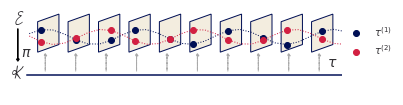
\includegraphics[width=.5\linewidth]{figures/math/fiberbundle.png}
  
    \caption{ The fiber $F$ is a continuous plane encoding the set of all possible (time, temperature) values.  The base space $K$ expresses that the fibers lie in continous space and therefore the data is continuous. The mapping $\pi:E\rightarrow K$ from total space to base space is what defines this structure as a fiber bundle. The continuous function $\tau_1$ returns a record in each fiber for each point on $K$; the set of all values $\tau_1$ returns is a dataset that lies in this fiberbundle. \note{remove one of the sections from this figure/maybe kill this example}}
    \label{fig:data_base_space} 
\end{figure}
The fiber bundle in figure~\ref{fig:data_base_space} is a representation of continuous (temperature, time) data. The fiber bundle abstraction facilitates seperately representing the time and temperature variables in the fiber $F$ and how these variables are connected in the base space $K$.  The function $\tau_1$ returns a record (temperature, time) for ever point on the interval $K$ and there can be many $\tau$ functions in the fiber bundle. 
